\chapter{全同粒子}\label{ch:b3:identical-particles}

宇宙中的每一个电子都严格、完全地与其他每一个电子全同——
不是像同一造币厂铸出的两枚硬币那样相似，
而是原则上不可区分：没有标签，
没有划痕，也没有历史能够标记其中任何一个。
量子力学对此极为认真，其后果支配着整个世界。
交换两个\omterm{def:b3:identical-particles:exchange}{全同粒子}不能改变任何可观测的东西，
因此多粒子波函数只有两种选择：
保持不变（\emph{玻色子}），或改变符号（\emph{费米子}）。
仅由负号便可导出泡利不相容原理、壳层结构
与整个元素\omterm{prop:b3:identical-particles:periodic}{周期表}，导出脚下物质的坚硬，
以及支撑起死亡恒星的压强；由正号则导出光子的群聚性——
激光由此而来——以及再过三章将出现的玻色–爱因斯坦凝聚。
物理学中很少有一个符号
承载如此之多的内容。

\section{对称化假设}

\begin{definition}[交换]\label{def:b3:identical-particles:exchange}
\index{全同粒子}\index{交换算符}
对于两个全同粒子，其态空间由乘积态
$\ket{a}\otimes\ket{b}$ 张成（粒子 1 处于 $\ket a$，粒子 2 处于
$\ket b$——位置、自旋等均包括在内），\emph{交换算符}
$\hat P_{12}$ 交换两者的角色：$\hat P_{12}\ket a\otimes\ket b =
\ket b\otimes\ket a$。它是厄米的，平方为单位算符，并且
与任何对粒子作同样处理的\omterm{def:b3:hamiltonian-mechanics:hamiltonian}{哈密顿量}对易；
其\omterm{def:b3:quantum-formalism:observable}{本征值} $\pm1$ 是世界中守恒的标记。
\end{definition}

\begin{theorem}[玻色子与费米子]\label{thm:b3:identical-particles:postulate}
\index{玻色子}\index{费米子}\index{自旋–统计定理}
\omterm{def:b3:identical-particles:exchange}{全同粒子}的态不仅被允许，而且
\emph{必须}是每一种交换的本征态：对于一类粒子——\emph{玻色子}——态完全
\emph{对称}，对于另一类粒子——\emph{费米子}——态完全\emph{反对称}
（每次交换都改变符号）。
某一物种属于哪一类，
由其自旋决定（\emph{自旋–统计定理}，
仅在相对论量子场论中得到证明，此处予以承认）：
\[
\text{整数自旋} \Rightarrow \text{玻色子} , \qquad
\text{半整数自旋} \Rightarrow \text{费米子} .
\]
光子、π 介子和 $^4$He 原子是玻色子；电子、质子、
中子和 $^3$He 是费米子。
复合粒子的行为与其组成部分之和相同：偶数个费米子束缚在一起
是玻色子（$^4$He：2p + 2n + 2e），奇数个则是费米子
（$^3$He）——其后果之明显，
犹如两种不同的液态氦。
\end{theorem}
\admitted

\begin{corollary}[泡利不相容原理]\label{cor:b3:identical-particles:pauli}
\index{泡利不相容原理}
两个费米子永远不能占据同一个单粒子态：取 $\ket a = \ket b$ 代入
反对称组合 $(\ket a\otimes\ket b - \ket b\otimes\ket a)/\sqrt2$，
得到零矢量——
这样的态不存在。对于电子（自旋 $\tfrac12$），
每个轨道至多容纳两个电子，且自旋投影相反。
\end{corollary}

\begin{example}[不同的计数方式]\label{ex:b3:identical-particles:counting}
两个粒子分布于两个态 $a, b$ 中：经典（可区分）
计数给出四种构型；玻色子有三种（$aa$、$bb$，
以及\emph{一}种混合态）；费米子恰有一种（混合的、
反对称的那一种）。统计物理将整体继承这些计数
（\cref{ch:b3:quantum-statistics}）；在此已能
消解十九世纪的一个尴尬难题——同一种气体的
两份样品“混合”时的熵
（\cref{exo:b3:identical-particles:10}）。
\end{example}

\section{周期表}

\begin{proposition}[壳层，以及化学存在的原因]\label{prop:b3:identical-particles:periodic}
\index{周期表}\index{构造原理}
依次将每个类氢轨道 $(n, l, m, m_s)$ 各填入一个电子，
按能量由低到高，能级次序由穿透与屏蔽决定
（$1s$、$2s$、$2p$、$3s$、$3p$、$4s$、$3d$、\dots ——
\cref{exo:b3:hydrogen-atom:8}）。泡利原理使填充达到
\emph{饱和}：$2$ 个电子填满第一壳层，$8$ 个电子填
满第二和第三行，元素\omterm{prop:b3:identical-particles:periodic}{周期表}由此获得
其周期。化学研究的是不相容原理留给最外层的
那些电子：满壳层（稀有气体）是惰性的；
多出一个电子于满壳层之外（碱金属），或差一个电子才满壳层
（卤素），两者以相反的方式具有反应性。若没有负号，
每个电子都会下沉到 $1s$，每个原子都会变成
缩小的类氦小球，于是既没有化学键，
也没有分子，也就没有化学家为此遗憾。
\end{proposition}
\admitted

\begin{omfigure}
\begin{tikzpicture}[font=\small, >=Stealth]
  % 1s
  \draw[thick] (0,0) rectangle (1.0,0.7);
  \node[anchor=north] at (0.5,-0.08) {$1s$};
  \node at (0.5,0.35) {$\uparrow\downarrow$};
  % 2s
  \draw[thick] (1.9,0) rectangle (2.9,0.7);
  \node[anchor=north] at (2.4,-0.08) {$2s$};
  \node at (2.4,0.35) {$\uparrow\downarrow$};
  % 2p: three boxes
  \foreach \i in {0,1,2} \draw[thick] ({3.5+\i*1.05},0) rectangle ({4.5+\i*1.05},0.7);
  \node[anchor=north] at (5.05,-0.08) {$2p$（三个轨道）};
  \node at (4.0,0.35) {$\uparrow\downarrow$};
  \node at (5.05,0.35) {$\uparrow$};
  \node at (6.1,0.35) {$\uparrow$};
  \node[anchor=west, align=left, font=\footnotesize] at (7.4,0.35)
    {氧（$Z = 8$）：$1s^2\,2s^2\,2p^4$\\
     平行自旋的电子先分占各轨道 \\ （洪特规则）};
  \draw[decorate, decoration={brace, mirror, amplitude=4pt}] (0,-0.65) -- (2.9,-0.65);
  \node[font=\footnotesize] at (1.45,-1.05) {He、Be 处壳层闭合};
  \draw[decorate, decoration={brace, mirror, amplitude=4pt}] (3.5,-0.65) -- (6.55,-0.65);
  \node[font=\footnotesize] at (5.05,-1.05) {Ne 处壳层闭合：第二行结束};
\end{tikzpicture}

{\small 两两填充轨道：泡利不相容原理
决定了\omterm{prop:b3:identical-particles:periodic}{周期表}的周期。氧的四个 $2p$ 电子
说明洪特规则——自旋平行地先分占各个轨道
之后才配对，这纯属交换效应
（\cref{prop:b3:identical-particles:exchange-force}）。}
\end{omfigure}

\section{交换相互作用}

\begin{proposition}[双电子空间态的对称性]\label{prop:b3:identical-particles:exchange-force}
\index{交换相互作用}
对于两个电子，总态（空间 $\times$ 自旋）必须是
反对称的：一个\emph{单态}（反对称自旋，
\cref{exo:b3:spin-two-level:11}）迫使空间波函数为\emph{对称}的，
而\emph{三重态}则迫使其反对称。两者的物理意义不同：
物理上二者的区别在于：在反对称的空间态中，电子
永不重合（$\psi(\vect r, \vect r) = 0$），彼此保持分开；
而对称态则允许它们聚集。由于靠近需要付出库仑能，
自旋排布便获得一个能量差——
即\emph{交换能}——其量级为静电能（电子伏特！），
但并不存在如此强度的磁力：自旋平行或反平行
是几何与排斥共同作用的结果。这正是洪特规则、
氦的两套光谱、共价键的根源，以及——
经晶体放大后，铁磁性本身的根源
（见\cref{ch:b3:electromagnetism-in-matter}）。
\end{proposition}

\begin{proof}[部分证明]
对称性的核算由
\cref{thm:b3:identical-particles:postulate}加上自旋组合给出；
重合处为零，是反对称性在
$\vect r_1 = \vect r_2$ 处的体现。能量结果来自排斥作用的一阶
\omterm{thm:b3:perturbation-theory:corrections}{微扰理论}：直接项对两种对称性都相同，
而“交换”积分以相反的符号进入
（见\cref{exo:b3:identical-particles:6}）。
\end{proof}

\begin{omfigure}
\begin{tikzpicture}
  \begin{axis}[omaxis, axis x line=bottom, axis y line=left,
    width=11.4cm, height=5.4cm, xmin=-3.4, xmax=3.4, ymin=0, ymax=1.28,
    xlabel={分离距离 $x_1 - x_2$（任意单位）},
    ylabel={双粒子概率密度},
    xlabel style={at={(axis description cs:0.5,-0.1)}, anchor=north},
    xtick=\empty, ytick=\empty, clip=false,
    legend style={font=\scriptsize, at={(0.98,0.76)}, anchor=north east,
      draw=none, fill=none}]
    \addplot[omThm, very thick, domain=-3.4:3.4, samples=120]
      {(1+exp(-x*x))*exp(-x*x/6)*0.62};
    \addlegendentry{对称（玻色子；单态电子）}
    \addplot[omDef, very thick, domain=-3.4:3.4, samples=120]
      {(1-exp(-x*x))*exp(-x*x/6)*0.9};
    \addlegendentry{反对称（三重态电子）}
  \end{axis}
\end{tikzpicture}

{\small 在间距 $x_1 - x_2$ 处找到该粒子对的概率：
对称空间态在接触处聚集，反对称态
则带有“交换空穴”——重合处严格为零。
将此几何结构代入库仑排斥，自旋排布
便获得电子伏特量级的能量差。}
\end{omfigure}

\begin{example}[同一原子中的两种氦]\label{ex:b3:identical-particles:helium}
氦的激发态 $1s\,2s$ 分为两族，彼此几乎不发生跃迁：
\emph{仲氦}（单态，空间对称）与
\emph{正氦}（三重态，空间反对称），其能级
\emph{更低}，约 $\approx\qty{0.8}{eV}$——其交换空穴
避开了库仑排斥。基态必然是仲氦（$1s^2$
要求空间对称态）；而最低的正氦态，
既无更低的三重态可供衰变，自旋翻转又被禁戒，
寿命可达数小时——这种亚稳原子是原子束实验的主力。
十九世纪的光谱学家曾编目过“两种氦”；
其解答只是一个负号。
\end{example}

\begin{example}[共价键]\label{ex:b3:identical-particles:bond}
将两个氢原子靠近：两个电子可以进入两个原子轨道的
对称空间组合（自旋
为单态），或反对称组合（三重态）。对称态
将电荷堆积在两质子\emph{之间}，在此处同时吸引两者：
形成束缚——即 H$_2$ 的共价键，深度为 \qty{4.5}{eV}。
反对称态则将中平面清空：纯粹排斥。
有机化学的每一条规则，都是对自旋成对的电子
作对称共享的记账——泡利不相容原理反过来运用，
正是分子的粘合剂。
\end{example}

\section{玻色子：越多越好}

\begin{proposition}[玻色增强]\label{prop:b3:identical-particles:enhancement}
\index{受激辐射!玻色子起源}
使已含 $n$ 个玻色子的态再增加一个玻色子的跃迁
其振幅增强为 $\sqrt{n + 1}$ 倍——速率增强为 $n + 1$ 倍
（阶梯代数见\cref{ch:b3:harmonic-oscillator}，因为
玻色模式\emph{本身}即是振子）。“$1$”项是自发辐射；
“$n$”项则是\emph{受激}辐射，正比于
已有的粒子数：每台激光器背后的雪崩
（本科二年级分册），如今揭示为纯粹的交换对称性。同一
统计规律，用于冷却到波包相互重叠的原子时，
预言粒子会一拥而入同一个量子态——
玻色–爱因斯坦凝聚，
留待在\cref{ch:b3:quantum-statistics}中讨论。
\end{proposition}
\admitted

\begin{method}[处理全同粒子]\label{met:b3:identical-particles:method}
(1) 由自旋决定统计性质（复合粒子：加上
费米子数）。(2) 对两个电子，将空间 $\times$ 自旋因子化，
并使单态与对称空间配对，三重态与反对称空间配对。
(3) 计数态，而不是给粒子编名：列出占据数。
(4) 涉及排斥的能量问题：直接积分计算一次，交换
积分取对称性所对应的符号。(5) 记住两条口诀——
费米子：每个态至多一个，每个粒子周围有交换空穴；
玻色子：速率随占据数增强。
\end{method}

\begin{omfigure}
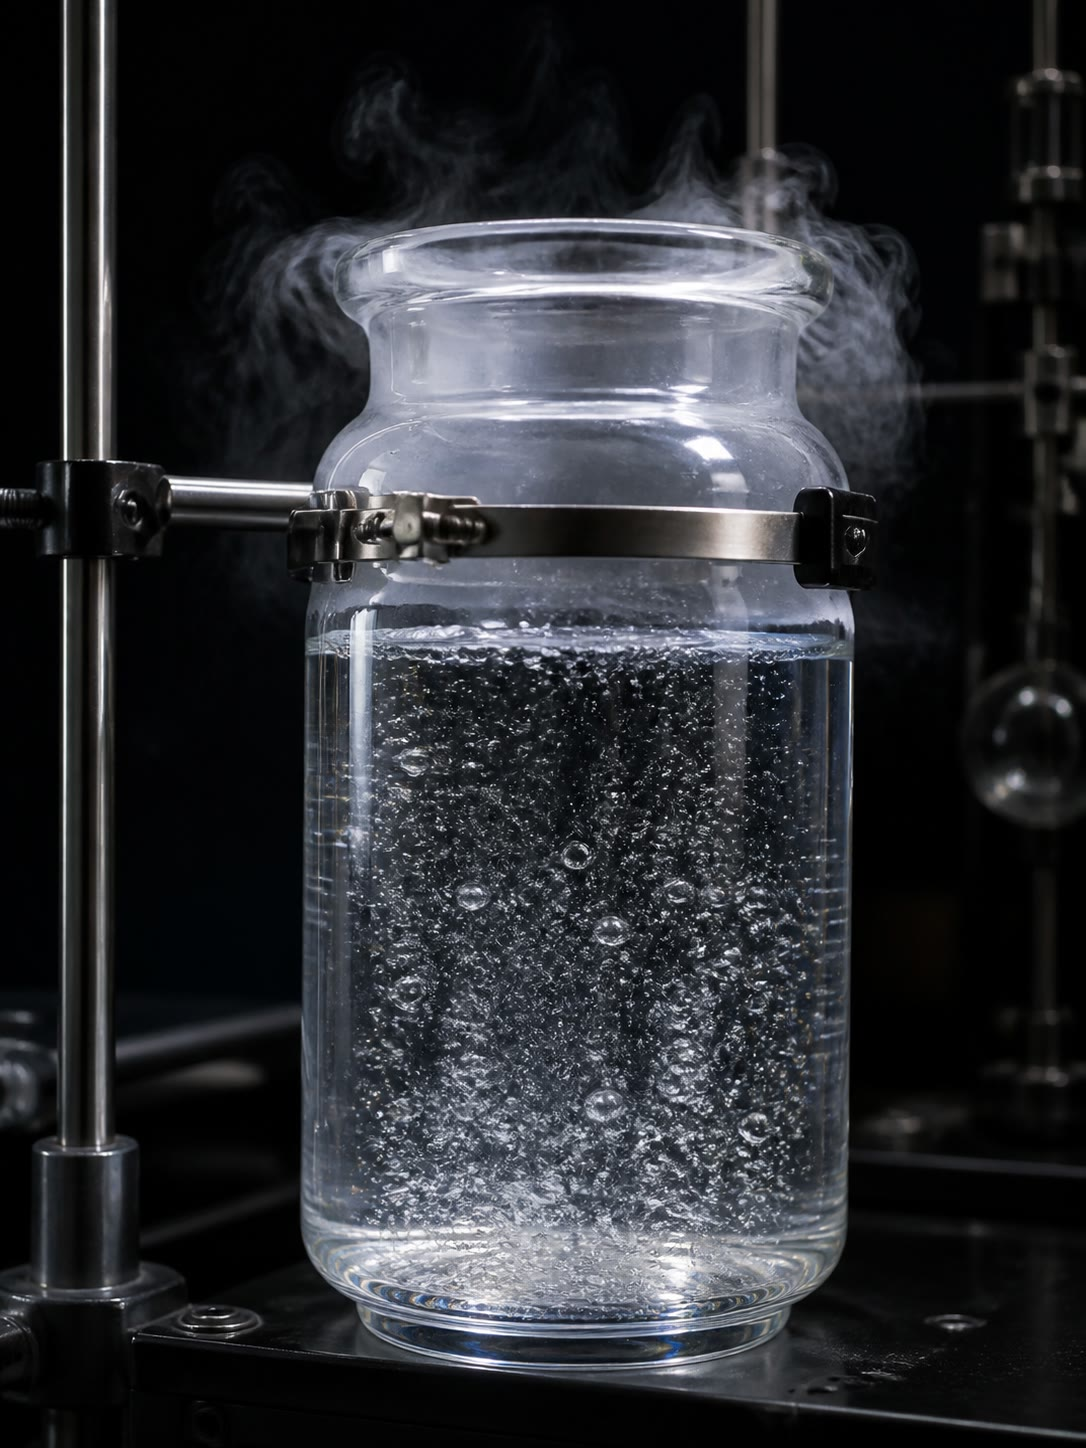
\includegraphics[width=0.45\linewidth]{images/book5/ai/b5-14-liquid-helium-dewar.jpg}

{\small 液氦在 \qty{4}{K} 附近安静地沸腾：一种由完全相同的玻色子组成的流体。再低几度，它便突然停止沸腾，并无摩擦地流动——全同性被提升到流体力学层面。}
\end{omfigure}

\section{练习}

\begin{exercise}[$\star$]\label{exo:b3:identical-particles:1}
(a) 证明 $\hat P_{12}$ 是厄米的，且 $\hat P_{12}^2 = \mathbb 1$：
其可能的\omterm{def:b3:quantum-formalism:observable}{本征值}是什么？(b) 证明 $[\hat P_{12}, \hat H] =
0$（对\omterm{def:b3:identical-particles:exchange}{全同粒子}），并断定对称类型
守恒。(c) 为何两个\omterm{def:b3:identical-particles:exchange}{全同粒子}的态不能
简单地“是” $\ket a\otimes\ket b$ 而不具任何对称性？(d) 对下列各项分类：
$^1$H、$^2$H（氘）、$^4$He、$^3$He、氢分子、一个
光子。
\end{exercise}

\begin{exercise}[$\star$]\label{exo:b3:identical-particles:2}
(a) 写出由正交
轨道 $\ket a, \ket b$ 构成的归一化反对称态。(b) 证明当 $a = b$ 时它为零。(c)
对处于 $a, b, c$ 态的三个费米子，写出完全反对称组合（共六项，符号正负交替——
即一个 $3\times3$ 行列式），并验证交换一次会使其变号。(d) 为何
行列式形式
使泡利原理自动成立？
\end{exercise}

\begin{exercise}[$\star$]\label{exo:b3:identical-particles:3}
两个粒子共享三个正交态。计算两粒子态的数目，
分别对 (a) 可区分粒子；(b) 玻色子；(c) 费米子
（无自旋）。(d) 对带自旋的电子重复 (c)：
现在有多少个态？
\end{exercise}

\begin{exercise}[$\star$]\label{exo:b3:identical-particles:4}
(a) 给出碳、氮、氧和
氖的基态电子组态。(b) 叙述洪特规则，并将其用于氮的三个 $2p$
电子。(c) 用一句话，由
\cref{prop:b3:identical-particles:exchange-force}论证洪特规则。(d) 哪种元素的满壳层使其
成为已知最不活泼的物质，
而缺少哪一个电子又使氟成为最活泼的元素？
\end{exercise}

\begin{exercise}[$\star\star$]\label{exo:b3:identical-particles:5}
能级为 $E_n = n^2E_1$ 的盒中两个无相互作用粒子。
(a) 求两个玻色子的基态能量；两个无自旋费米子的基态能量；两个
电子的基态能量。(b) 分别求各自的第一激发能级。
(c) 费米子的基态能量更高：这种“费米抬升”是
萌芽状态的压强——用一句话解释它如何阻止物质
坍缩。(d) 推广：盒中 $N$ 个无自旋费米子——
证明基态能量按 $N^3$ 增长，而非 $N$。
\end{exercise}

\begin{exercise}[$\star\star$]\label{exo:b3:identical-particles:6}
设 $\varphi_a, \varphi_b$ 为正交实轨道，
双粒子态 $\psi_\pm \propto \varphi_a(1)\varphi_b(2) \pm
\varphi_b(1)\varphi_a(2)$：(a) 证明 $\psi_-(\vect r, \vect r) = 0$；
(b) 推导
$\langle(\vect r_1 - \vect r_2)^2\rangle_\pm =
(\text{公共项}) \mp 2\,|\bra{a}\hat{\vect r}\ket{b}|^2$，
并指出哪种对称性使粒子相距更远；(c) 对
排斥相互作用 $V(|\vect r_1 - \vect r_2|)$，论证
$E_+ - E_-$ 的符号；(d) 与氦的正、仲态能级次序相联系。
\end{exercise}

\begin{exercise}[$\star\star$]\label{exo:b3:identical-particles:7}
氦的能级阶梯。(a) 为何基态必须是自旋单态？
(b) $1s2s$ 三重态比
$1s2s$ 单态低 \qty{0.80}{eV}：将其表示为交换积分，并比较其
大小与磁自旋–自旋能（$\sim\mu_{\text{B}}^2\mu_0/4\pi
a_0^3$，并估算其值）。(c) 为何 $2\,^3S$ 态是亚稳的
（哪两条选择定则必须同时被破坏？）(d) 其实测寿命
为 $\approx\qty{8000}{s}$，请与
氢 $2p$ 态的 \qty{1.6}{ns} 比较，并审慎地感叹一番。
\end{exercise}

\begin{exercise}[$\star\star$]\label{exo:b3:identical-particles:8}
正氢与仲氢。H$_2$ 的两个质子是费米子：
\emph{总}核自旋 $\times$ 转动态必须
在交换下反对称；交换质子还会使分子轴反向，
使转动态乘以
$(-1)^J$。(a) 证明核自旋三重态（正氢）与奇数 $J$ 配对，
核自旋单态（仲氢）与偶数 $J$ 配对。(b) 在高温下，
由自旋多重度决定的正、仲比值为何？(c) 正氢的
最低态（$J = 1$）比仲氢高出 $2B \approx \qty{15}{meV}$，
即高于仲氢的 $J = 0$ 态，而自旋转换需要数天：
在刚液化的氢储罐中，随正氢份额缓慢转化，会发生什么，
以及为何液化厂必须在
储存\emph{之前}催化这一转化？(d) 哪种日常低温燃料
方案（火箭！）恰好遇到这一问题？
\end{exercise}

\begin{exercise}[$\star\star$]\label{exo:b3:identical-particles:9}
玻色子的奔涌。一个模式容纳 $n$ 个光子；添加一个光子的矩阵元
按 $\sqrt{n+1}$ 变化。(a) 证明射入该模式的发射速率
按 $n + 1$ 标度，吸收速率按 $n$ 标度。(b) 在一个谐振腔中，
其中一个模式容纳 $10^{10}$ 个光子，相邻模式中没有光子，
比较一个激发原子射入各模式的发射速率。(c) 用两句话解释
这一机制如何使激光在单一
模式中\emph{增长}。(d) 在\cref{prop:b3:harmonic-oscillator:coherent-motion}中
$\sqrt{n+1}$ 是否已经出现过？
\end{exercise}

\begin{exercise}[$\star\star\star$]\label{exo:b3:identical-particles:10}
由全同性解决的吉布斯佯谬。两份相等体积 $V$ 的
理想气体，各含 $N$ 个分子，温度相同，将它们连通。(a) 若
两种气体\emph{不同}（例如氩与氖），熵
增加 $2Nk_{\text{B}}\ln2$——回忆其原因（每种气体的
体积都加倍）。(b) 若二者是\emph{同一种}气体，打开阀门
宏观上没有任何变化：若混合熵仍然出现，
将导致什么荒谬结论（考虑关闭再重新打开）？
(c) 证明把分子视为可区分粒子
\emph{确实}会产生虚假熵，并证明将态数
除以 $N!$——这仅因分子全同才合理——
即可消除它。(d) 用一句话概括其寓意：经典统计物理
悄悄借用了一个量子事实；后续章节
将大张旗鼓地借用它。
\end{exercise}

\begin{exercise}[$\star\star\star$]\label{exo:b3:identical-particles:11}
泡利撑起了逝去的恒星。一颗白矮星的密度约为
$\qty{e9}{kg/m^3}$，即电子数密度 $n_{\text{e}} \approx
\qty{3e35}{m^{-3}}$（每两个核子质量对应一个电子）。(a)
利用
\cref{exo:b3:schrodinger-three-dimensions:8}
求费米能——并注意非相对论公式已显勉强。(b) 比较
$E_{\text{F}}$ 与 $k_{\text{B}}T$（取 $T = \qty{e7}{K}$），这颗白热恒星在何种
意义上是\emph{冷}的？(c) 用两句话说明
泡利不相容（而非热）如何提供
与引力平衡的压强。(d) 质量增加，
$E_{\text{F}}$ 转为相对论性，必然发生什么——
这预示着哪一著名极限（见\cref{ch:b3:astrophysics}）？
\end{exercise}

\begin{exercise}[$\star\star\star$]\label{exo:b3:identical-particles:12}
由交换到磁铁。将固体中两个相邻电子
用\cref{prop:b3:identical-particles:exchange-force}描述，其
能量为 $E_{\text{单态}}$ 或 $E_{\text{三重态}} =
E_{\text{单态}} - 2J$，交换常数为 $J$。(a) 证明该能量可由
有效自旋\omterm{def:b3:hamiltonian-mechanics:hamiltonian}{哈密顿量} $\hat H =
-2J\,\hat{\vect S}_1\cdot\hat{\vect S}_2/\hbar^2$（利用
$\hat{\vect S}_1\cdot\hat{\vect S}_2 = \tfrac12[\hat S^2 - \hat
S_1^2 - \hat S_2^2]$）。(b) 当 $J > 0$ 时相邻自旋取向一致：
由此类自旋对组成的晶格会产生何种宏观现象？
(c) 估算有序温度 $k_{\text{B}}T_{\text{C}}
\sim J$，取 $J \approx \qty{0.1}{eV}$，并与铁的
\qty{1043}{K}比较。(d) 为何\emph{磁}偶极–偶极
相互作用（回忆其大小，见
\cref{exo:b3:identical-particles:7}b）无法解释千开尔文的磁铁——
那么何物可以？请用一句话回答。
\end{exercise}

\section{问题：元素周期表的逻辑}

\begin{problem}[{周末问题——三条量子规则构建
全部化学}]\label{pb:b3:identical-particles:1}
只需给一位物理学家氢原子轨道 $(n, l, m)$、电子自旋
与泡利不相容原理，\omterm{prop:b3:identical-particles:periodic}{周期表}便随之而来——
周期、族、原子大小、电离能的锯齿形起伏，乃至
金的颜色。本题即由此构建。数据：类氢
能级 $-13.6\,Z_{\text{有效}}^2/n^2$ eV；实测第一电离
能（eV）：H $13.6$、He $24.6$、Li $5.4$、Be $9.3$、B $8.3$、
C $11.3$、N $14.5$、O $13.6$、F $17.4$、Ne $21.6$、Na $5.1$。

\medskip\noindent\textbf{第一部分——三条规则。}
\begin{enumerate}
  \item 陈述三要素：轨道目录
        $(n, l, m)$ 及其简并度、自旋二重性和
        泡利不相容原理。$n = 1$、
        $2$、$3$ 各能容纳多少个电子？
  \item 为何多电子原子中亚壳层的\emph{能量次序}
        与氢原子仅按 $n$ 排列的次序不同？
        （回忆穿透与屏蔽，
        见\cref{exo:b3:hydrogen-atom:8}）？
  \item 写出直到 $4s$ 和 $3d$ 的填充次序，并给出
        Na（$Z = 11$）、Cl（$17$）、K（$19$）的电子组态，
        Fe（$26$）的电子组态。
  \item 周期长度：由填充次序解释观测到的 $2, 8, 8, 18$
        \omterm{prop:b3:identical-particles:periodic}{周期表}前四个周期的长度（为何第三行是
        8，而非 18？）。
  \item 何种单一特征使稀有气体在化学上
        表现为惰性？
  \item 定义价电子所感受的有效电荷 $Z_{\text{有效}}$，
        并说明为何钠的外层电子约为 $1$，而
        氦的两个电子各自所见
        几乎为完整的 $Z = 2$ 减去彼此
        屏蔽的一部分。
\end{enumerate}

\medskip\noindent\textbf{第二部分——读懂第二行。}
\begin{enumerate}[resume]
  \item 由数据可见，电离能自 Li 到 Ne 上升，但
        在 B 与 O 处出现下降，请定位这两处。
  \item 解释硼处的下降（哪一亚壳层于 B 处开始填充，以及为何
        $2p$ 比 $2s$ 更难容纳？）。
  \item 解释氧处的下降（氧的两个 $2p$ 电子
        首次须做何事，以及哪条规则所带来的
        稳定性丧失？）。
  \item 若粗略估计氦的电离能为
        $13.6 \times Z^2 = \qty{54.4}{eV}$，而实测值
        \qty{24.6}{eV} 为何小得多，并且
        拟合得出的 $Z_{\text{有效}} \approx 1.34$ 说明了什么？
  \item 锂的 \qty{5.4}{eV} 与氢的 \qty{13.6}{eV} 相比，
        哪两种效应（屏蔽；更高的 $n$）共同起作用？
  \item 为何沿一行原子\emph{尺寸}随之缩小
        （Li $\to$ Ne），尽管不断添加电子？
\end{enumerate}

\medskip\noindent\textbf{第三部分——族与化学键。}
\begin{enumerate}[resume]
  \item 碱金属：稀有气体芯之上的一个 $s$ 电子——由此组态推导
        其族特征（低电离能、$+1$ 价离子、剧烈的
        与水的反应）。
  \item 卤素：$p$ 壳层上有一个空穴——推导其
        族特征（电子亲和能、$-1$ 价离子、双原子分子）。
  \item 碳的四价：为何 $2s^22p^2$ 原子在实际中
        呈四价（何种近简并使其能够激发并
        杂化——回忆
        \cref{ex:b3:perturbation-theory:stark}中的斯塔克杂化）？
  \item 利用\cref{ex:b3:identical-particles:bond}：为何两个闭壳层原子
        （即两个氦原子）\emph{不}
        形成共价键？
  \item 过渡金属：$4s$/$3d$ 近简并使得十列
        化学性质相近，为何填充
        \emph{内层} $d$ 壳层时化学性质改变如此之小？
  \item 仅由电子组态预测，K、Ca、Sc 中
        哪一元素首先出现具备磁性的未成对 $d$ 电子。
\end{enumerate}

\medskip\noindent\textbf{第四部分——超越经验法则。}
\begin{enumerate}[resume]
  \item 洪特规则赋予氮原子三个平行的 $2p$ 自旋：
        这固定了哪一可测的原子性质（即其磁矩），
        而第 14 章中的哪一机制提供了
        这种取向所需的能量？
  \item \omterm{prop:b3:identical-particles:periodic}{周期表}本身的存在要求电子严格全同：
        若电子只是“略有区别”，
        泡利原理与壳层闭合将受到什么影响？
  \item 在重原子中，内层电子以 $Z\alpha c$ 运动：
        对于金（$Z = 79$），估算 $v/c$，其对象为 $1s$ 电子对，
        并定性说明相对论对 $6s$
        轨道能量的影响——这是被普遍接受的解释，
        可说明金的颜色和汞的液态性质。
  \item $4s$ 支壳层先于 $3d$ 填充，却在过渡金属中
        \emph{先}电离，铬和铜会借用一个 $s$ 电子，
        以达到 $3d^5$ 和 $3d^{10}$：
        这些反常现象说明两个支壳层的能量
        彼此靠得有多近？
  \item 同一元素的两种同位素在化学上几乎完全相同：
        由三条规则出发，为何化学只关心 $Z$，
        而几乎不关心原子核的质量？
  \item 第 7 周期止于 $Z \approx 118$ 附近，超重元素化学
        偏离了\omterm{prop:b3:identical-particles:periodic}{周期表}朴素的族列逻辑：
        请指出两个相互竞争的尺度：壳层结构，
        以及大 $Z$ 下的相对论效应与库仑效应。
  \item 总结这一命名结果：一套轨道目录、一次自旋加倍、一个负号——
        其结果即周期律：各周期所含元素数为 $2, 8, 8, 18$，
        B 与 O 处的凹陷，活泼元素与惰性元素各自成族，
        这些均可在电离阶梯中测得，
        阶梯从 \qty{5.1}{eV}（Na）到
        \qty{24.6}{eV}（He）。
\end{enumerate}
\end{problem}
